\documentclass{../../slides-style}

\slidetitle{Лекция 3: Моделирование как инструмент архитектуры}{06.03.2025}

\begin{document}

    \begin{frame}[plain]
        \titlepage
    \end{frame}

    \section{Модели}

    \begin{frame}
        \frametitle{Моделирование}
        \begin{itemize}
            \item \textbf{Модель} --- упрощённое подобие объекта или явления
            \item Нужны для изучения некоторых их свойств, абстрагируясь от сложности ``настоящего'' объекта или явления
            \item Модели используются повсеместно
            \begin{itemize}
                \item Математические модели
                \item Модели как реальные объекты
                \item Модели в разработке ПО
            \end{itemize}
        \end{itemize}
    \end{frame}

    \begin{frame}
        \frametitle{Общие свойства моделей}
        \begin{itemize}
            \item Содержат меньше информации, чем реальность
            \item Существуют для определённой цели
            \item Модели субъективны, что позволяет отделить существенные свойства от несущественных
            \item Моделирование ПО:
            \begin{itemize}
                \item Модели предназначены прежде всего для управления сложностью
                \item Позволяют понять, проанализировать и протестировать систему до её реализации
            \end{itemize}
        \end{itemize}

        \center{\textbf{All models are wrong, some are useful}}
    \end{frame}

    \begin{frame}
        \frametitle{Как выбрать, что моделировать?}
        \begin{itemize}
            \item При моделировании надо определиться с:
            \begin{itemize}
                \item Какие архитектурные решения нуждаются в моделировании
                \item На каком уровне детализации
                \item Насколько формально
            \end{itemize}
            \item Необходимо учитывать соотношение трудозатрат и выгоды
            \begin{itemize}
                \item Стоимость создания \textit{и поддержания} модели не должна быть больше преимуществ от её использования
            \end{itemize}
        \end{itemize}
        \begin{center}
            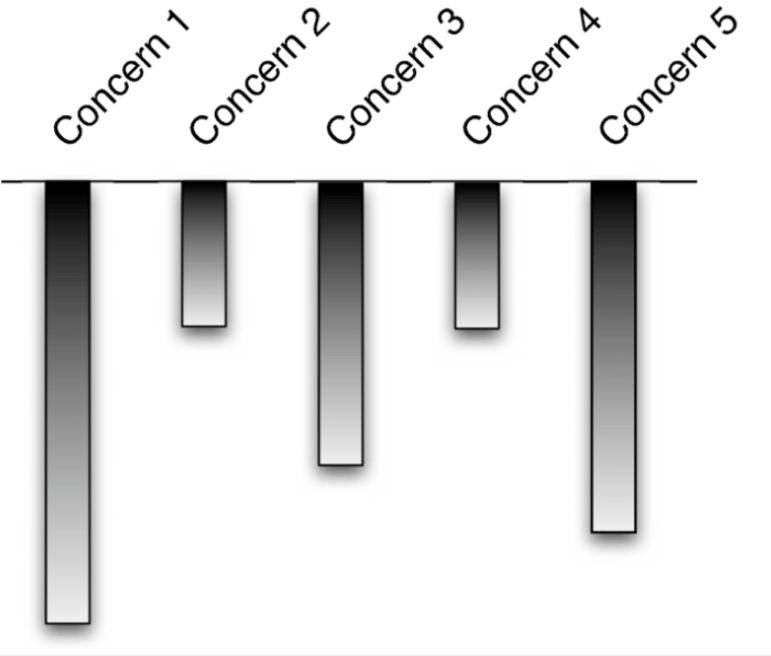
\includegraphics[width=0.4\textwidth]{concerns.png}
            \attribution{N. Medvidovic}
        \end{center}
    \end{frame}

    \section{Виды моделей}

    \begin{frame}
        \frametitle{Модели бывают разные}
        \begin{itemize}
            \item Используемые нотации и способы моделирования зависят от целей моделирования
            \begin{itemize}
                \item От неформальных набросков до исполнимых моделей
            \end{itemize}
        \end{itemize}
        \begin{center}
            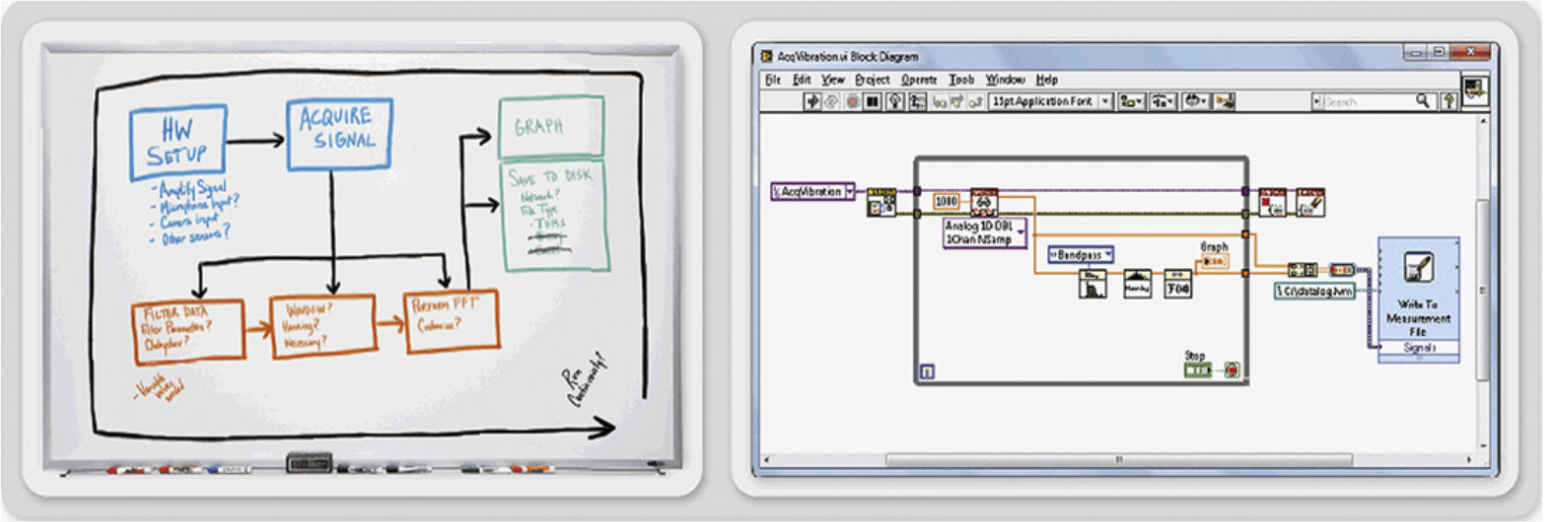
\includegraphics[width=0.9\textwidth]{sketchesVsFormalNotations.png}
            \attribution{N. Medvidovic}
        \end{center}
    \end{frame}

    \begin{frame}
        \frametitle{Виды моделей}
        \framesubtitle{Естественные языки}
        \begin{columns}
            \begin{column}{0.5\textwidth}
                \begin{itemize}
                    \item Обычный текст --- вполне себе инструмент моделирования
                    \item Очень выразителен, не требует специальных знаний, максимально гибок
                    \item Неоднозначен, неформален, не строг, слишком многословен, бесполезен для автоматической обработки
                \end{itemize}
            \end{column}
            \begin{column}{0.5\textwidth}
                \begin{center}
                    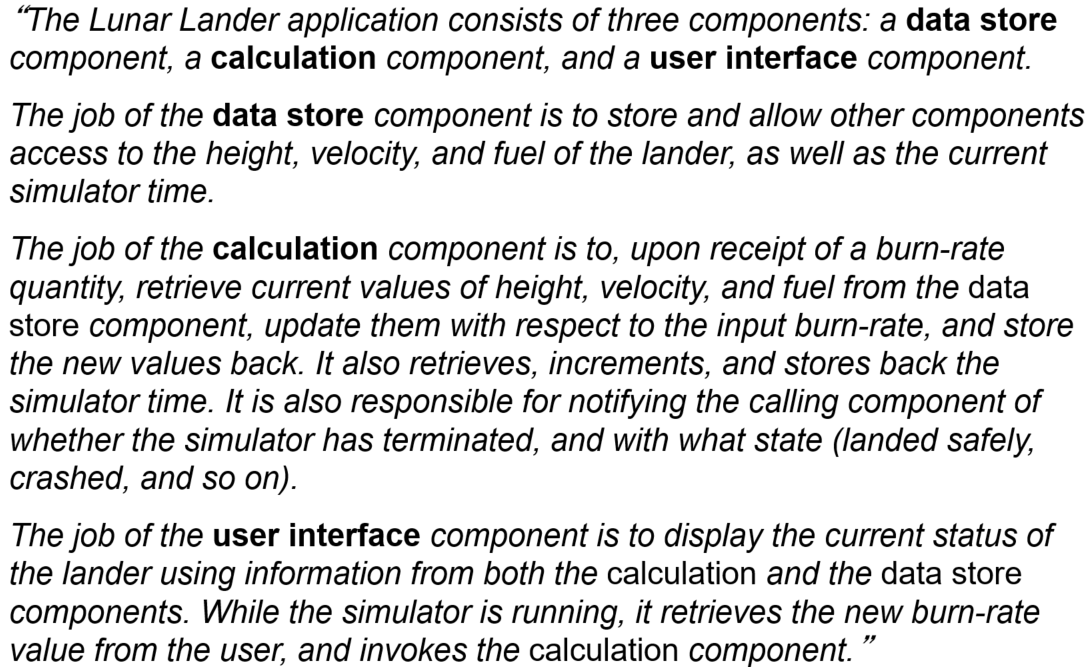
\includegraphics[width=\textwidth]{naturalLanguage.png}
                    \attribution{N. Medvidovic}
                \end{center}
            \end{column}
        \end{columns}
    \end{frame}

    \begin{frame}
        \frametitle{Неформальные графические модели}
        \begin{columns}
            \begin{column}{0.5\textwidth}
                \begin{itemize}
                    \item Диаграммы, рисуемые в PowerPoint, InkScape и подобном
                    \item Могут быть красивыми, как правило, простые, очень гибкая нотация
                    \item Неформальны, неоднозначны, не строги
                    \begin{itemize}
                        \item Но часто воспринимаются наоборот
                    \end{itemize}
                    \item Практически бесполезны для автоматической обработки
                \end{itemize}
            \end{column}
            \begin{column}{0.5\textwidth}
                \begin{center}
                    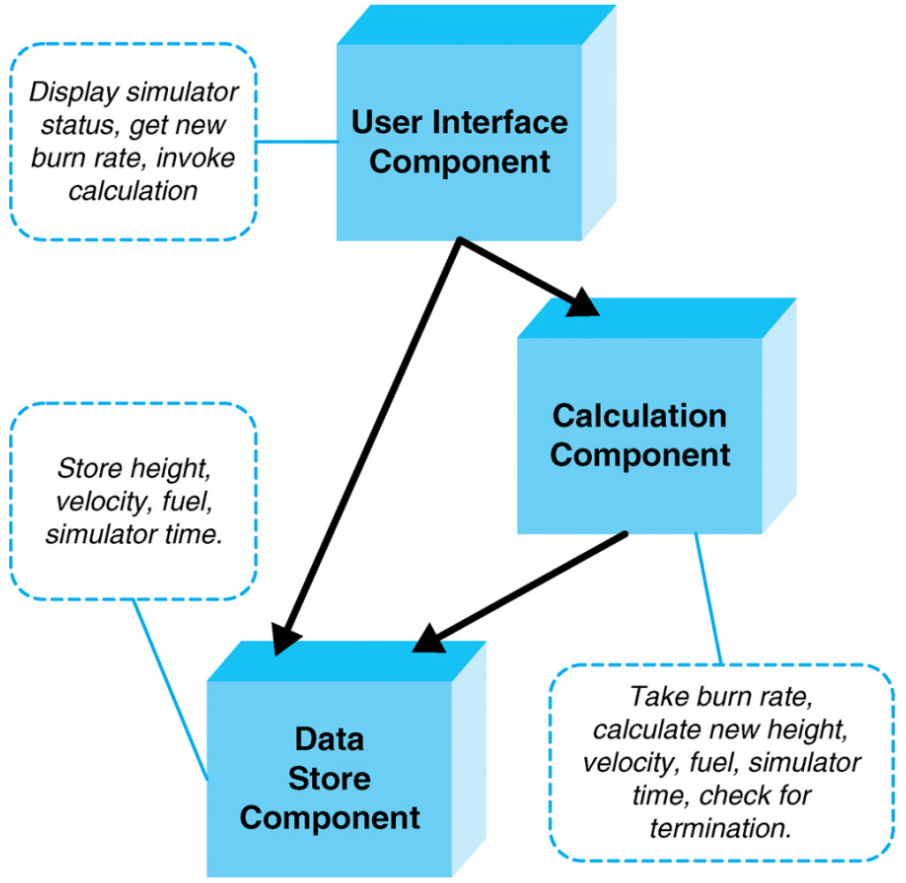
\includegraphics[width=0.9\textwidth]{informalModel.png}
                    \attribution{N. Medvidovic}
                \end{center}
            \end{column}
        \end{columns}
    \end{frame}

    \begin{frame}
        \frametitle{UML и SysML}
        \begin{columns}
            \begin{column}{0.4\textwidth}
                \begin{small}
                    \begin{itemize}
                        \item Несколько слабо связанных нотаций (``диаграмм'')
                        \item Поддерживают много точек зрения, общеприняты, широкая поддержка инструментами
                        \item Нет строгой семантики, сложно обеспечить консистентность, сложно расширять
                    \end{itemize}
                \end{small}
            \end{column}
            \begin{column}{0.6\textwidth}
                \begin{center}
                    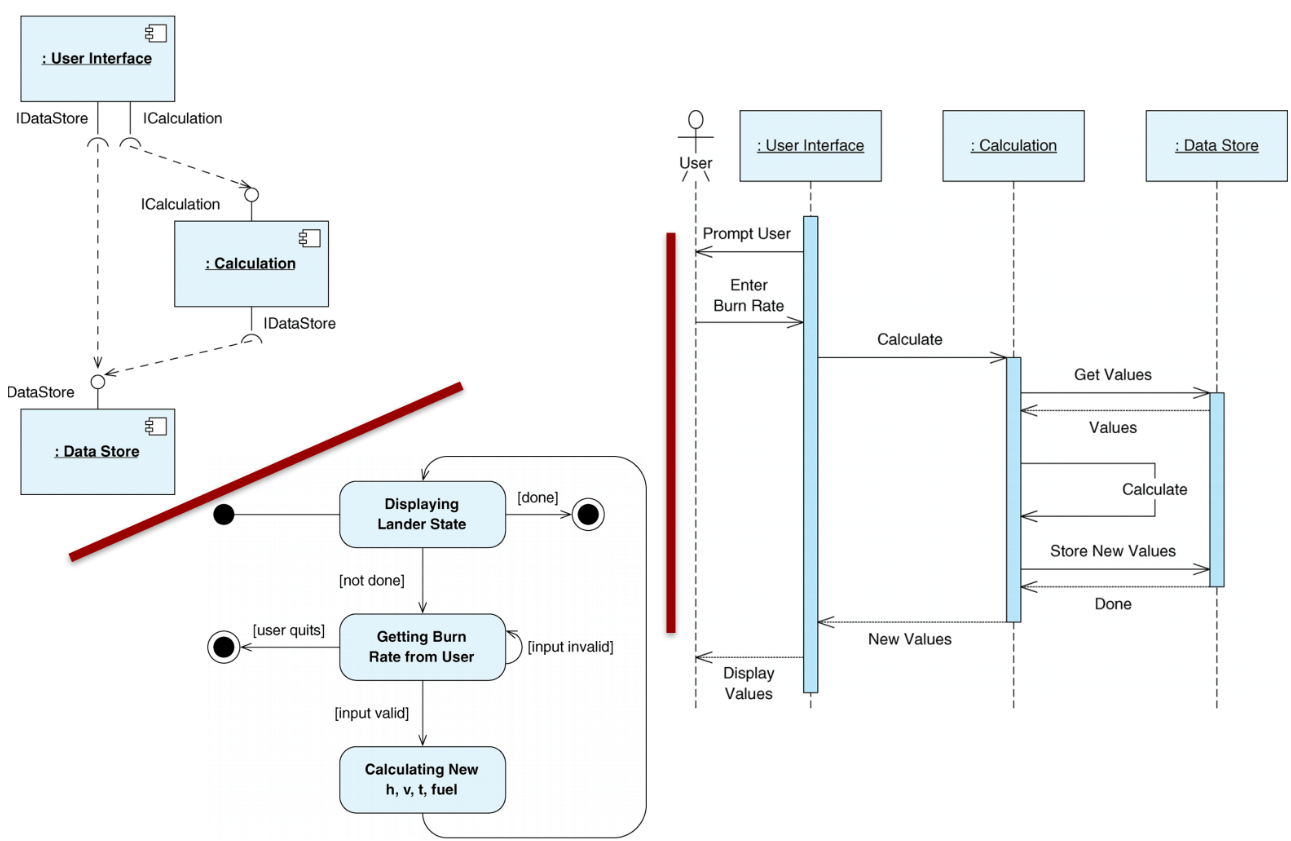
\includegraphics[width=\textwidth]{uml.png}
                    \attribution{N. Medvidovic}
                \end{center}
            \end{column}
        \end{columns}
    \end{frame}

    \begin{frame}
        \frametitle{AADL и другие текстовые формальные языки}
        \begin{columns}
            \begin{column}{0.4\textwidth}
                \begin{small}
                    \begin{itemize}
                        \item Хороши для моделирования встроенных систем и систем реального времени
                        \item Описывают одновременно ``железо'' и ``софт'', продвинутые инструменты анализа
                        \item Слишком многословны и детальны, сложны в изучении и использовании
                    \end{itemize}
                \end{small}
            \end{column}
            \begin{column}{0.6\textwidth}
                \begin{center}
                    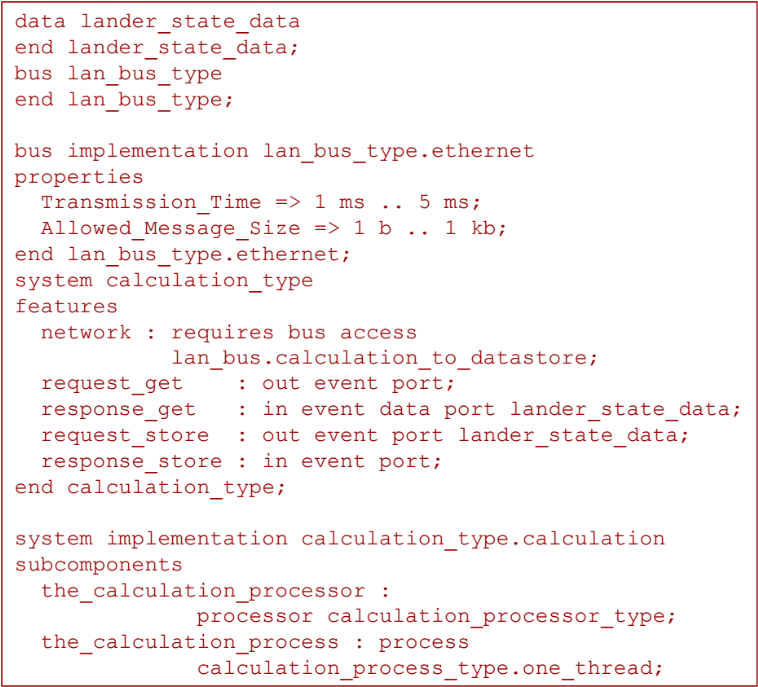
\includegraphics[width=0.85\textwidth]{aadl.png}
                    \attribution{N. Medvidovic}
                \end{center}
            \end{column}
        \end{columns}
    \end{frame}

    \section{UML}

    \begin{frame}
        \frametitle{Вернёмся к визуальным моделям}
        \begin{itemize}
            \item \textbf{Метафора визуализации} --- договорённость о том, как будут представляться сущности языка
            \item \textbf{Точка зрения моделирования} --- какой аспект системы и для кого моделируется
            \item Бывают одноразовые модели, документация и графические исходники
            \begin{itemize}
                \item \textbf{Семантический разрыв} --- неспособность модели полностью специфицировать систему
            \end{itemize}
        \end{itemize}
        \begin{center}
            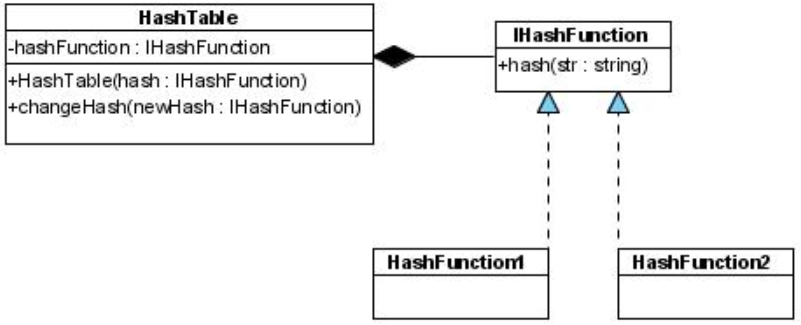
\includegraphics[width=0.5\textwidth]{hashTable.png}
        \end{center}
    \end{frame}

    \begin{frame}
        \frametitle{Unified Modeling Language}
        \begin{itemize}
            \item Семейство графических нотаций
            \begin{itemize}
                \item 14 видов диаграмм
            \end{itemize}
            \item Общая метамодель
            \item Стандарт под управлением Object Management Group
            \begin{itemize}
                \item UML 1.1 --- 1997 год
                \item UML 2.0 --- 2005 год
                \item UML 2.5.1 --- декабрь 2017 года
            \end{itemize}
            \item Прежде всего, для проектирования ПО
            \begin{itemize}
                \item После UML 2.0 стали появляться нотации и для инженеров
            \end{itemize}
            \item Расширяем
            \begin{itemize}
                \item Профили --- механизм легковесного расширения
                \item Метамоделирование
            \end{itemize}
        \end{itemize}
    \end{frame}

    \begin{frame}
        \frametitle{История}
        \begin{center}
            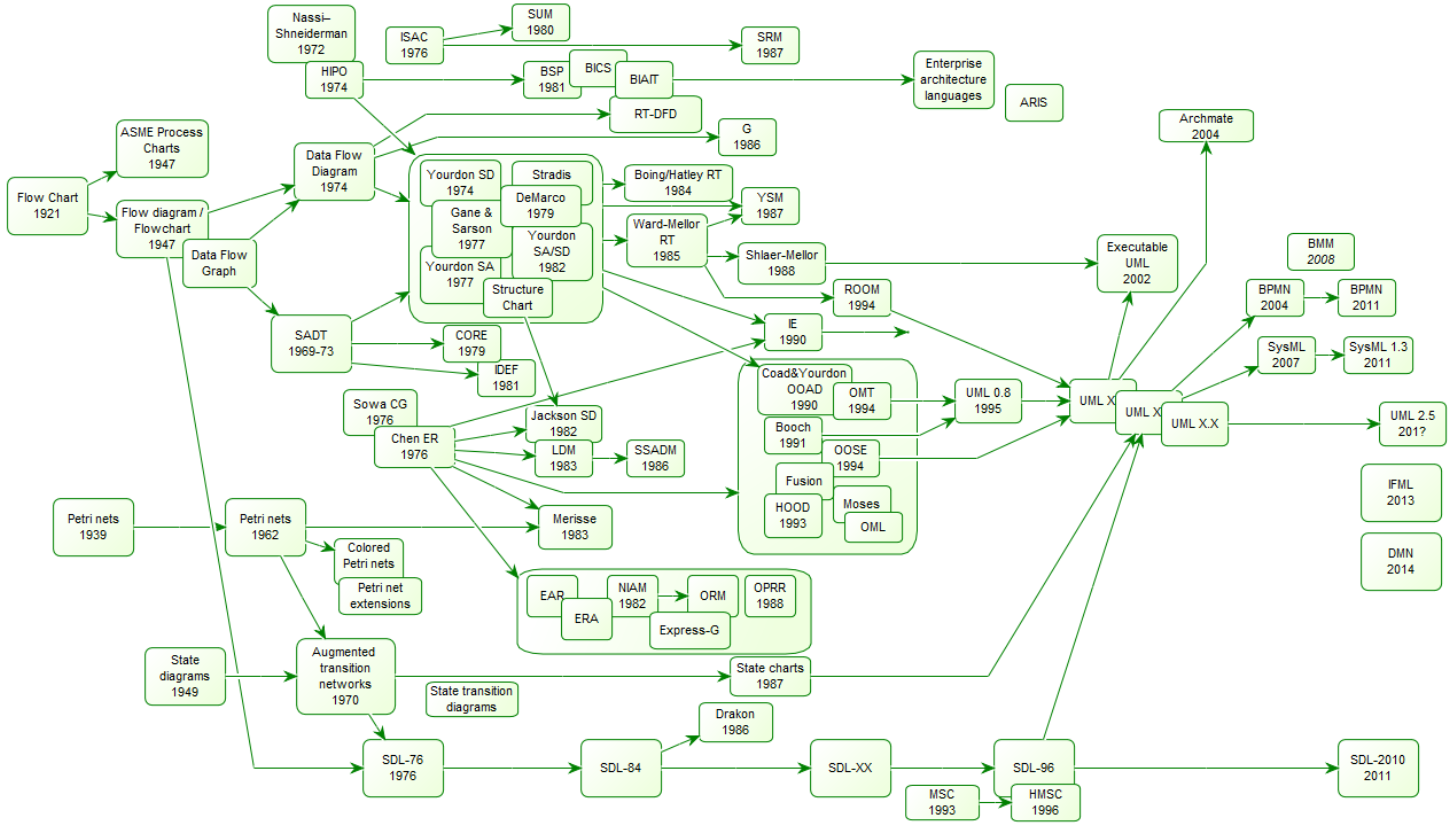
\includegraphics[width=\textwidth]{umlHistory.png}
        \end{center}
    \end{frame}

    \begin{frame}
        \frametitle{Виды диаграмм}
        \begin{center}
            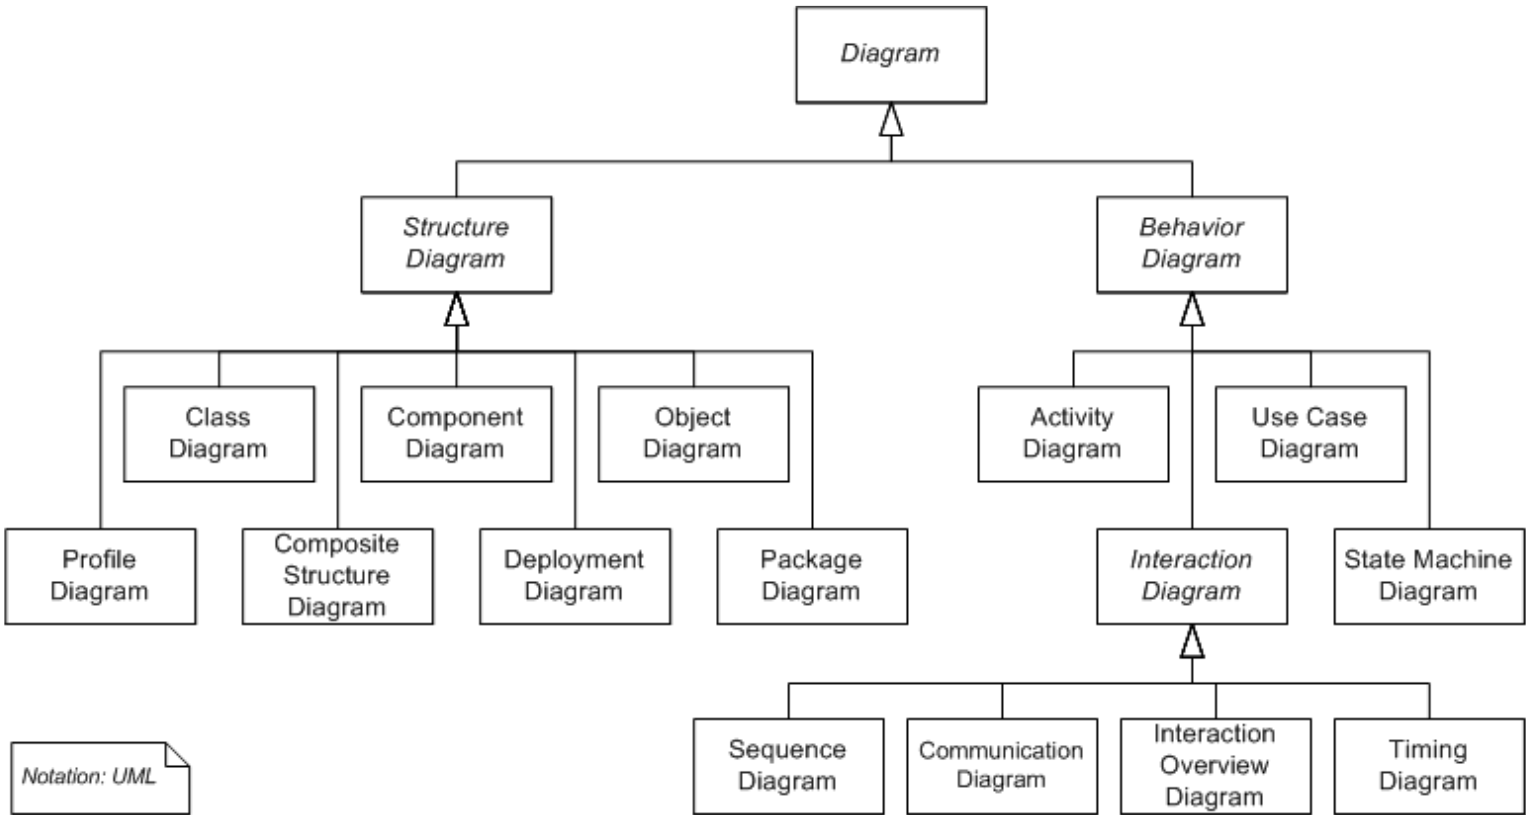
\includegraphics[width=\textwidth]{umlDiagrams.png}
        \end{center}
    \end{frame}

    \section{Диаграмма классов UML}

    \begin{frame}
        \frametitle{Диаграмма классов}
        \begin{center}
            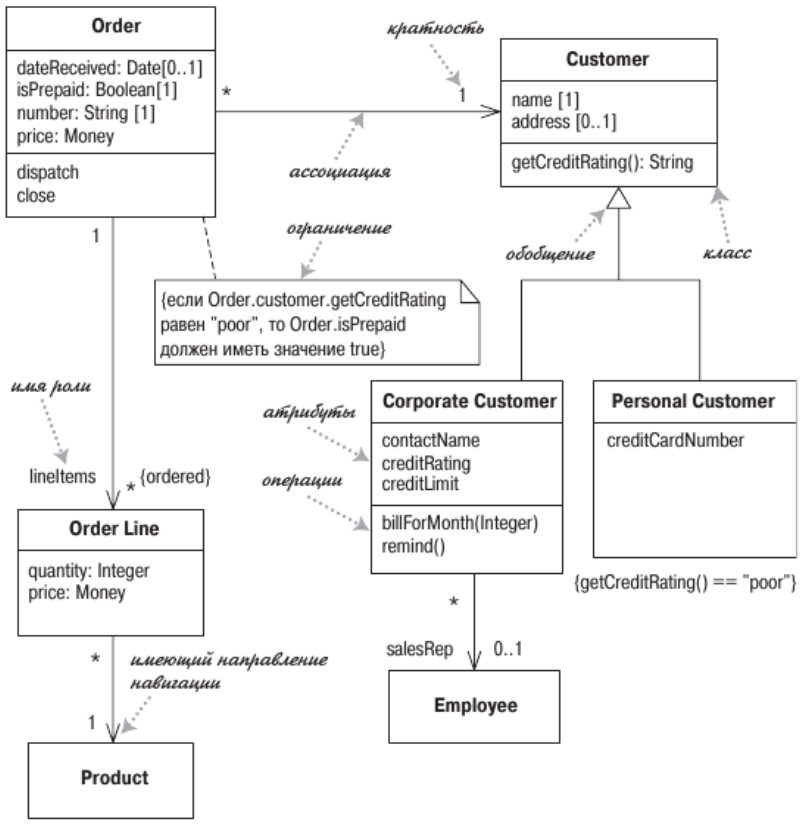
\includegraphics[height=0.8\textheight]{umlClassDiagram.png}
            \attribution{М. Фаулер. ``UML. Основы''}
        \end{center}
    \end{frame}

    \begin{frame}[fragile]
        \frametitle{Как это связано с кодом}
        \begin{columns}
            \begin{column}{0.5\textwidth}
                \begin{footnotesize}
                    \begin{minted}{java}
public class OrderLine {
    private int quantity;
    private Product product;
    public int getQuantity() {
        return quantity;
    }
    public void setQuantity(int quantity) {
        this.quantity = quantity;
    }
    public Money getPrice() {
        return product.getPrice().multiply(quantity);
    }
}
                    \end{minted}
                \end{footnotesize}
            \end{column}
            \begin{column}{0.5\textwidth}
                \begin{center}
                    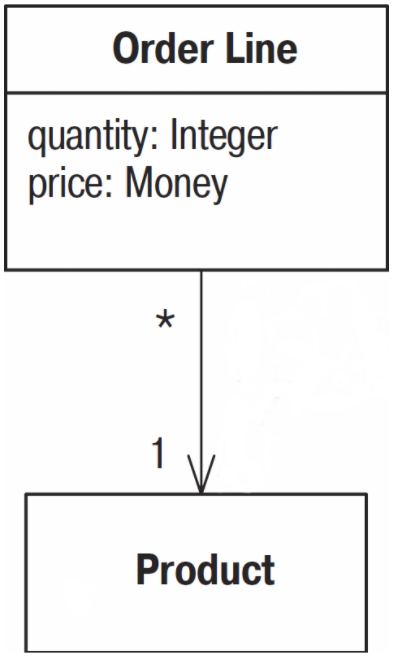
\includegraphics[width=0.5\textwidth]{orderLine.png}
                \end{center}
            \end{column}
        \end{columns}
    \end{frame}

    \begin{frame}[fragile]
        \frametitle{Двунаправленные ассоциации}
        \begin{columns}
            \begin{column}{0.5\textwidth}
                \begin{scriptsize}
                    \begin{center}
                        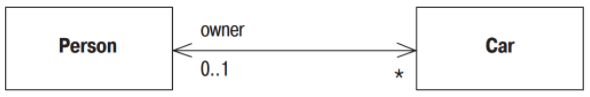
\includegraphics[width=0.9\textwidth]{twoWayAssociations.png}
                    \end{center}
    
                    \begin{minted}{csharp}
class Car {
    public Person Owner {
        get { return _owner; }
        set {
            if (_owner != null) 
                _owner.friendCars().Remove(this);
            _owner = value;
            if (_owner != null) 
                _owner.friendCars().Add(this);
        }
    }
    private Person _owner;
}
                    \end{minted}
                \end{scriptsize}
                \vspace{2mm}
            \end{column}
            \begin{column}{0.5\textwidth}
                \begin{scriptsize}
                    \begin{center}
                        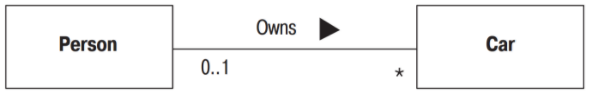
\includegraphics[width=0.9\textwidth]{personOwnsCar.png}
                    \end{center}
    
                    \begin{minted}{csharp}
class Person {
    public IList Cars {
        get { return ArrayList.ReadOnly(_cars); }
    }
    public void AddCar(Car arg) {
        arg.Owner = this;
    }
    private IList _cars = new ArrayList();
    internal IList friendCars() {
        // должен быть использован 
        // только Car.Owner
        return _cars;
    }
}
                    \end{minted}
                \end{scriptsize}
            \end{column}
        \end{columns}
    \end{frame}

    \begin{frame}
        \frametitle{Агрегация и композиция}
        Агрегация:
        \begin{center}
            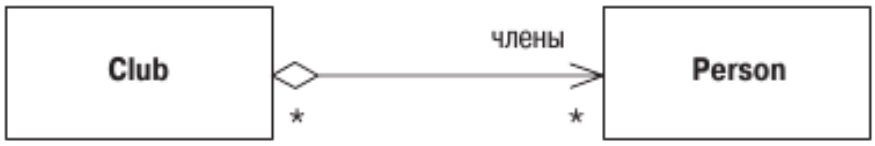
\includegraphics[height=0.1\textheight]{aggregation.png}
        \end{center}
        \vspace{5mm}
        Композиция:
        \begin{center}
            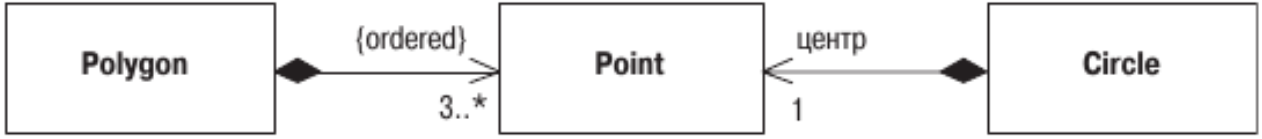
\includegraphics[height=0.1\textheight]{composition.png}
        \end{center}
        \attribution{М. Фаулер. ``UML. Основы''}
    \end{frame}

    \section{Диаграммы пакетов}

    \begin{frame}
        \frametitle{Диаграммы пакетов}
        \begin{center}
            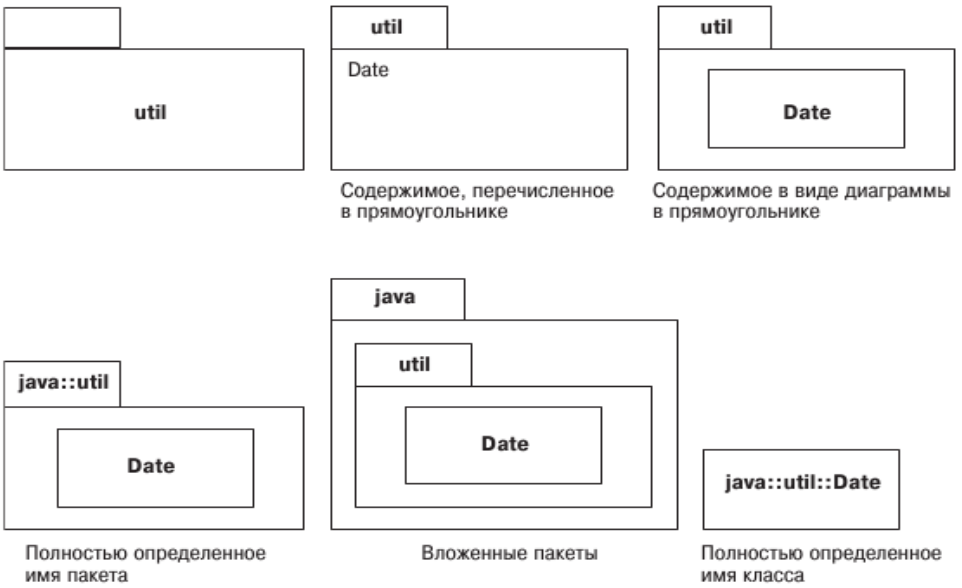
\includegraphics[width=0.8\textwidth]{packageDiagrams.png}
            \attribution{М. Фаулер. ``UML. Основы''}
        \end{center}
    \end{frame}

    \section{Диаграммы объектов}

    \begin{frame}
        \frametitle{Диаграммы объектов}
        \begin{center}
            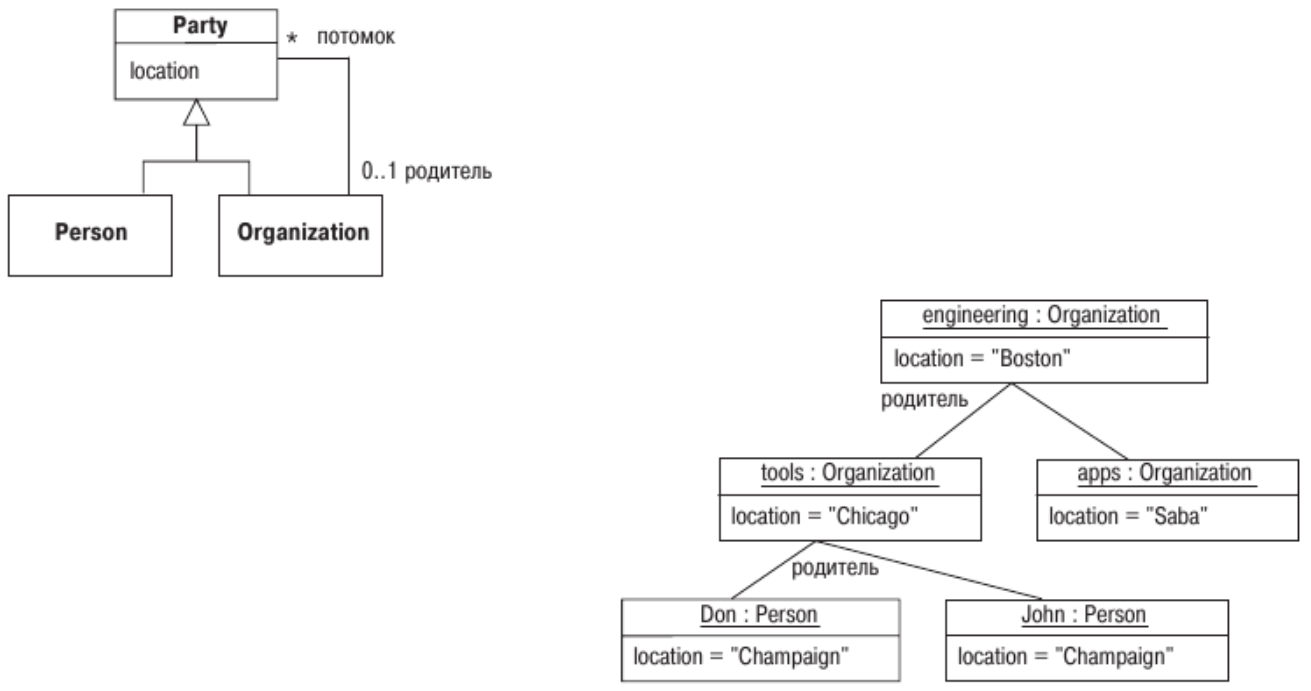
\includegraphics[width=0.9\textwidth]{objectDiagrams.png}
            \attribution{М. Фаулер. ``UML. Основы''}
        \end{center}
    \end{frame}

    \section{Диаграммы компонентов}
    
    \begin{frame}
        \frametitle{Диаграммы компонентов}
        \begin{center}
            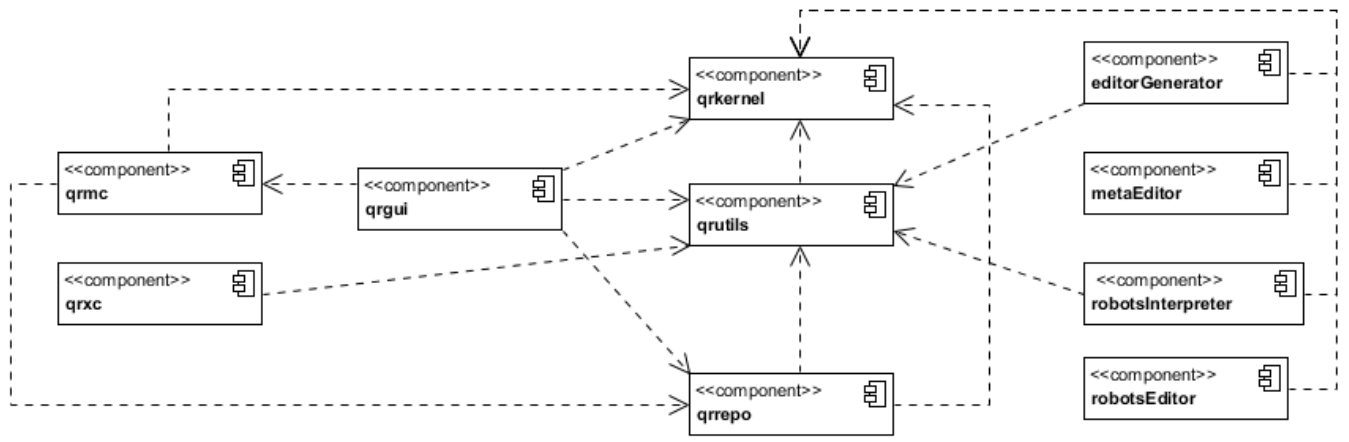
\includegraphics[width=0.95\textwidth]{componentDiagrams.png}
        \end{center}
    \end{frame}

    \begin{frame}
        \frametitle{Более подробно}
        \begin{center}
            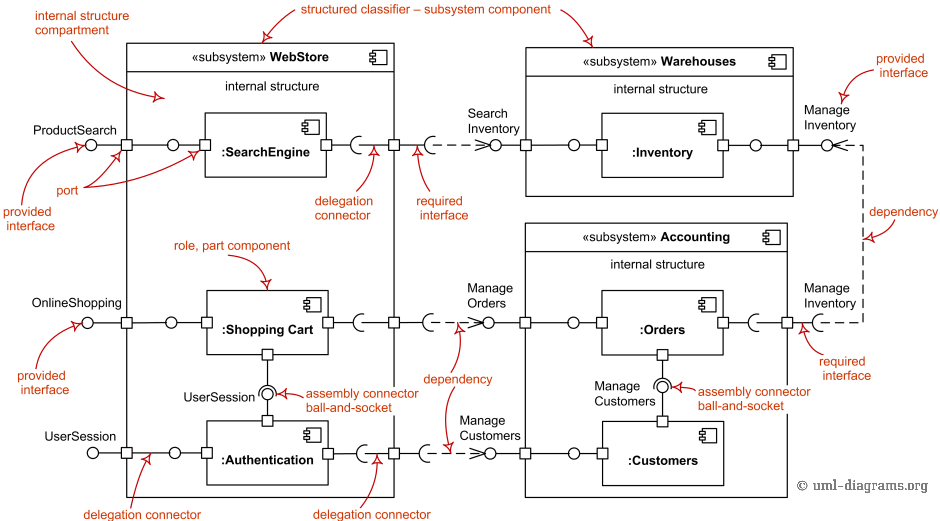
\includegraphics[width=0.95\textwidth]{componentDiagramsOverview.png}
            \attribution{\url{http://www.uml-diagrams.org}}
        \end{center}
    \end{frame}

    \begin{frame}
        \frametitle{Диаграмма случаев использования UML}
        \framesubtitle{Диаграмма прецедентов}
        \begin{columns}
            \begin{column}{0.5\textwidth}
                \begin{itemize}
                    \item Ивар Якобсон, 1992 год
                    \item Акторы (или актёры, роли) --- внешние сущности, использующие систему
                    \begin{itemize}
                        \item Люди или другие программные системы
                    \end{itemize}
                    \item Случаи использования (прецеденты)  --- цель использования системы актором
                    \begin{itemize}
                        \item Раскрываются в набор сценариев, описываемых чаще текстом
                    \end{itemize}
                \end{itemize}
            \end{column}
            \begin{column}{0.5\textwidth}
                \begin{center}
                    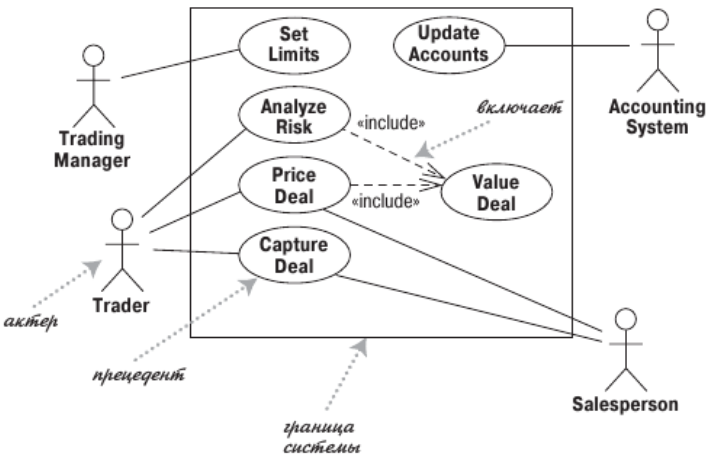
\includegraphics[width=\textwidth]{useCaseDiagram.png}
                    \attribution{М. Фаулер, UML. Основы}
                \end{center}
            \end{column}
        \end{columns}
    \end{frame}

    \begin{frame}
        \frametitle{Сценарий использования, типичная структура}
        \begin{itemize}
            \item Заголовок (цель основного актора)
            \item Заинтересованые лица, акторы, основной актор
            \item Предусловия
            \item Триггеры (активаторы)
            \item Основной порядок событий
            \item Альтернативные пути и расширения
            \item Постусловия
        \end{itemize}
    \end{frame}

    \begin{frame}
        \begin{center}
            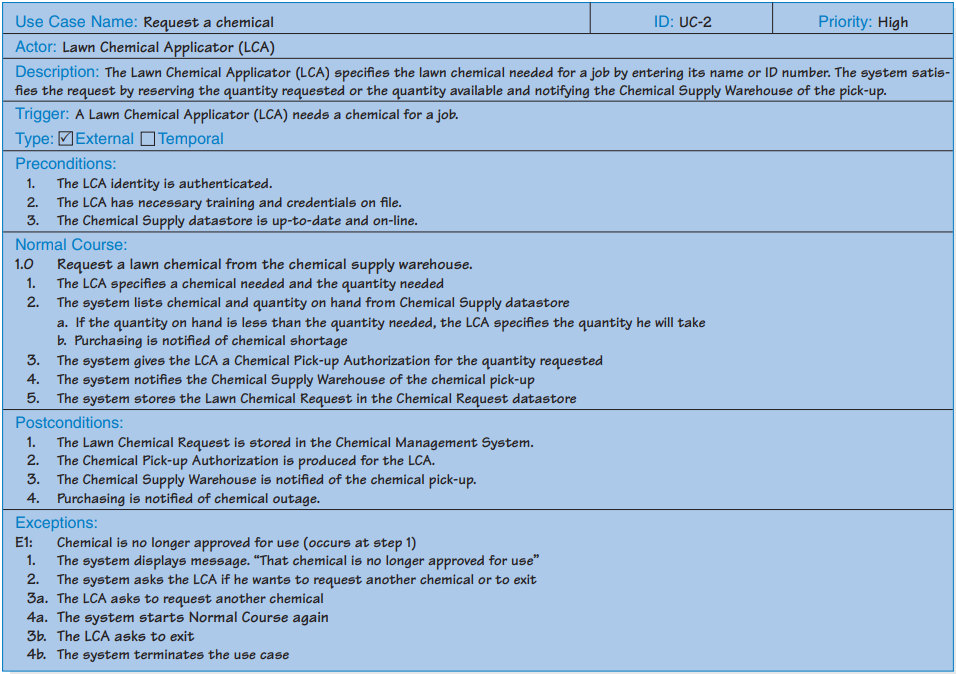
\includegraphics[width=0.9\textwidth]{useCaseExample.png}
            \attribution{R.M. Roth et al., System Analysis and Design}
        \end{center}
    \end{frame}

    \section{Диаграмма активностей UML}

    \begin{frame}
        \frametitle{Диаграмма активностей UML}
        \framesubtitle{Диаграммы деятельности}
        \begin{columns}
            \begin{column}{0.5\textwidth}
                \begin{itemize}
                    \item Используются для моделирования бизнес-процессов, тоже на первых этапах
                    \begin{itemize}
                        \item Может быть визуализацией сценария использования
                    \end{itemize}
                    \item Иногда --- для моделирования алгоритма
                    \item Расширенные блок-схемы
                    \item Семантика на основе сетей Петри
                \end{itemize}
            \end{column}
            \begin{column}{0.5\textwidth}
                \begin{center}
                    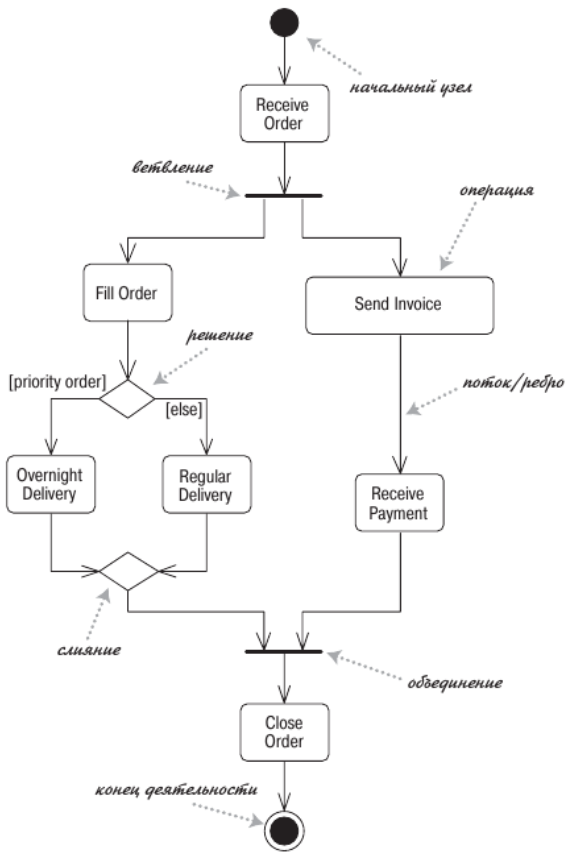
\includegraphics[width=0.7\textwidth]{activityDiagram.png}
                    \attribution{М. Фаулер, UML. Основы}
                \end{center}
            \end{column}
        \end{columns}
    \end{frame}

    \section{Диаграмма развёртывания}
    
    \begin{frame}
        \frametitle{Диаграмма развёртывания UML}
        \begin{columns}
            \begin{column}{0.5\textwidth}
                \begin{itemize}
                    \item Показывает отображение компонентов и физических артефактов на реальные (или виртуальные) устройства
                    \item Бывает полезна на начальных этапах проектирования, даже до диаграмм компонентов
                \end{itemize}
            \end{column}
            \begin{column}{0.5\textwidth}
                \begin{center}
                    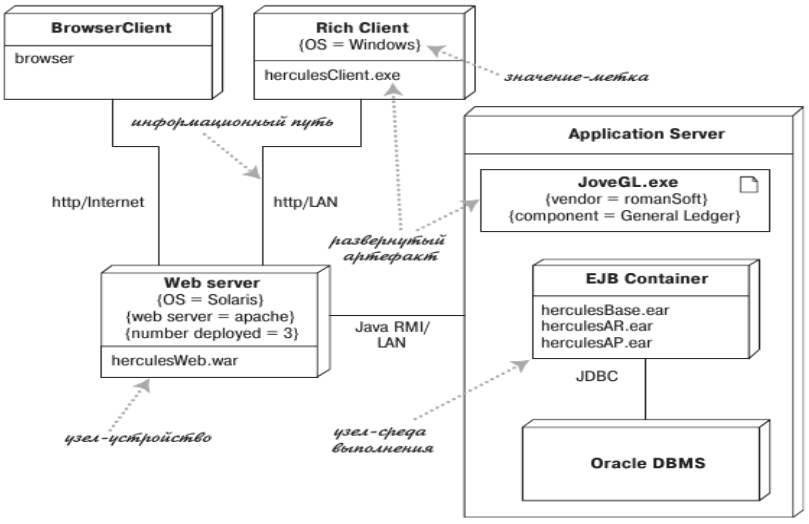
\includegraphics[width=\textwidth]{deploymentDiagram.png}
                    \attribution{М. Фаулер, UML. Основы}
                \end{center}
            \end{column}
        \end{columns}
    \end{frame}

    \section{Диаграммы ``Сущность-связь''}

    \begin{frame}
        \frametitle{Диаграммы ``Сущность-связь''}
        \begin{columns}
            \begin{column}{0.5\textwidth}
                \begin{itemize}
                    \item Описывают концептуальную модель предметной области
                    \item Идеальны для моделирования схем реляционных баз данных
                    \item 1976 год, Питер Чен
                \end{itemize}
            \end{column}
            \begin{column}{0.5\textwidth}
                \begin{center}
                    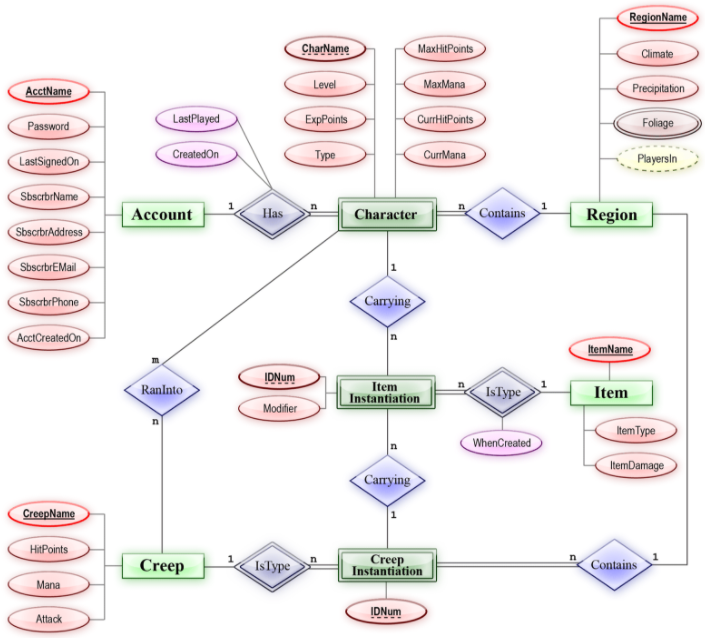
\includegraphics[width=\textwidth]{erChenNotation.png}
                    \attribution{https://ru.wikipedia.org}
                \end{center}
            \end{column}
        \end{columns}
    \end{frame}

    \begin{frame}
        \frametitle{Нотация ``Вороньей лапки''}
        \begin{center}
            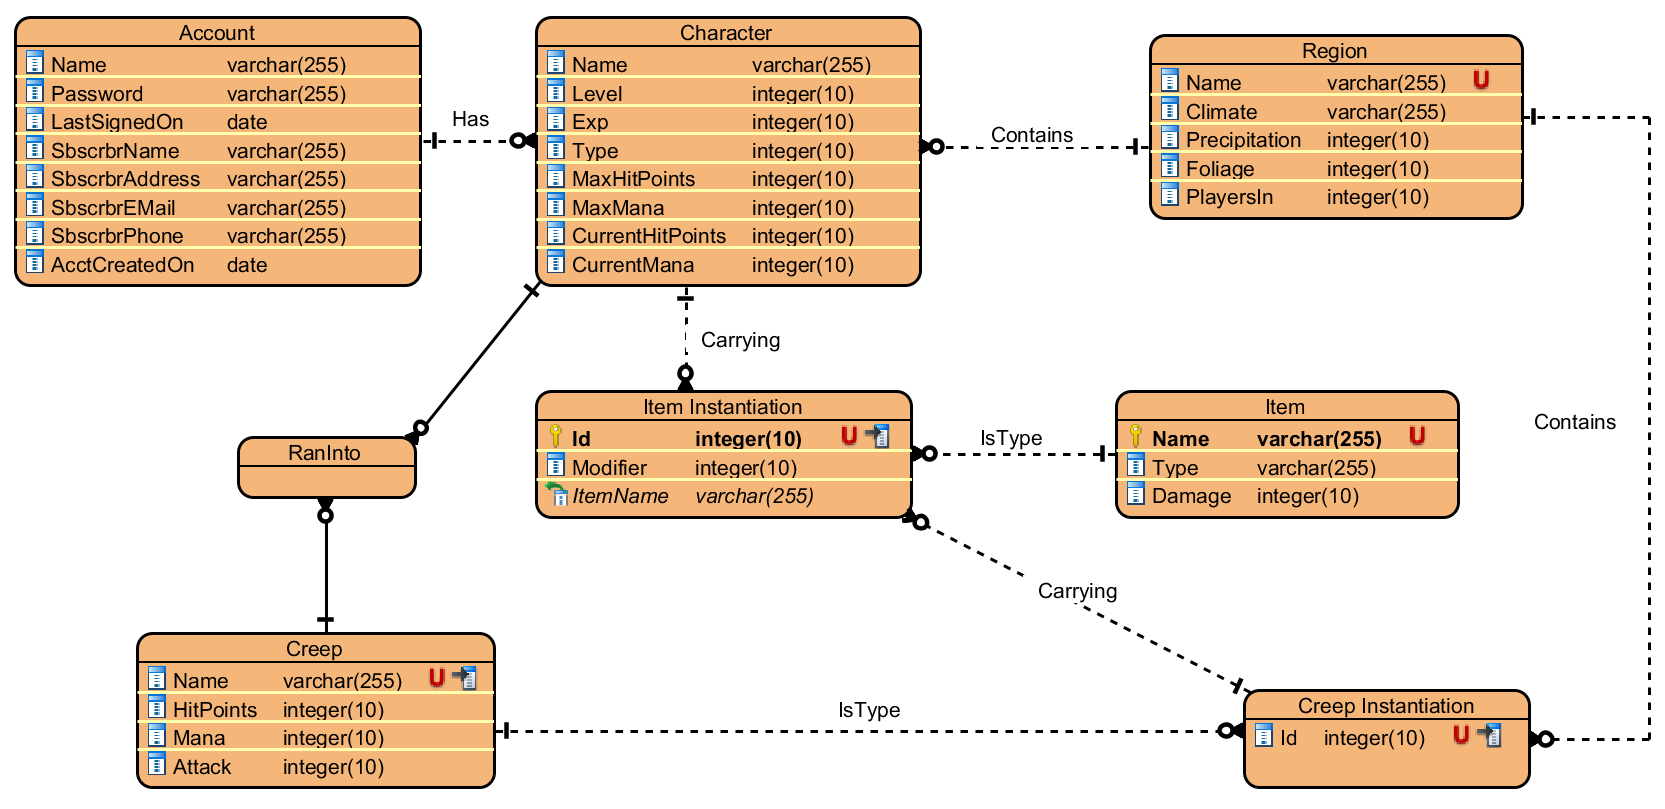
\includegraphics[width=\textwidth]{erCrowsFoot.png}
        \end{center}
    \end{frame}

    \section{Диаграммы конечных авоматов}

    \begin{frame}
        \frametitle{Диаграммы конечных автоматов}
        \framesubtitle{Диаграммы состояний}
        \begin{columns}
            \begin{column}{0.5\textwidth}
                \begin{itemize}
                    \item Состояния объекта как часть жизненного цикла
                    \item Моделирование реактивных объектов
                    \begin{itemize}
                        \item Например, сетевое соединение
                        \item Или знакомый пример с торговым автоматом
                    \end{itemize}
                    \item Имеют исполнимую семантику
                    \item Д. Харел, 1987
                \end{itemize}
            \end{column}
            \begin{column}{0.5\textwidth}
                \begin{center}
                    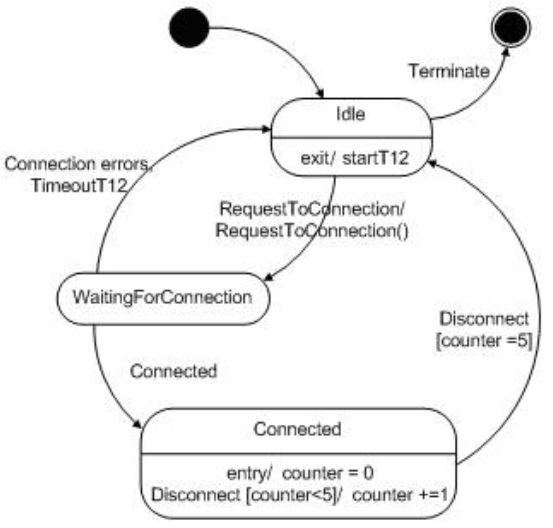
\includegraphics[width=0.7\textwidth]{stateTransitionExample.png}
                \end{center}
            \end{column}
        \end{columns}
    \end{frame}

    \begin{frame}
        \frametitle{Диаграммы конечных автоматов, особенности}
        Активности:
        \begin{columns}
            \begin{column}{0.5\textwidth}
                \begin{center}
                    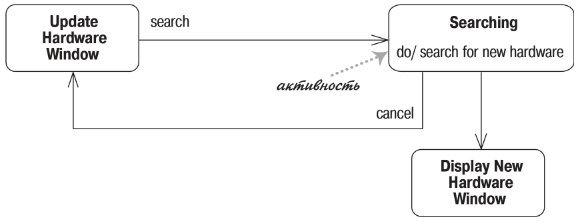
\includegraphics[width=\textwidth]{stateTransitionInternalEventExample.png}
                \end{center}
            \end{column}
            \begin{column}{0.5\textwidth}
                \begin{center}
                    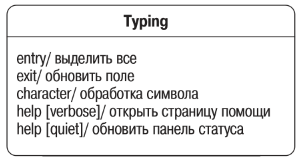
\includegraphics[width=0.5\textwidth]{stateTransitionInternalEvents.png}
                \end{center}
            \end{column}
        \end{columns}

        \begin{columns}
            \begin{column}{0.5\textwidth}
                Вложенные состояния:
                \begin{center}
                    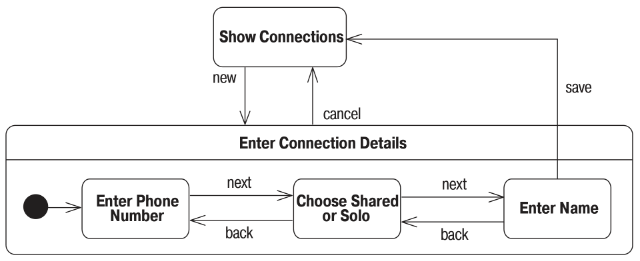
\includegraphics[width=\textwidth]{stateTransitionNestedStates.png}
                    \attribution{М. Фаулер, UML. Основы}
                \end{center}
            \end{column}
            \begin{column}{0.5\textwidth}
                Параллельные состояния, псевдосостояние истории:
                \begin{center}
                    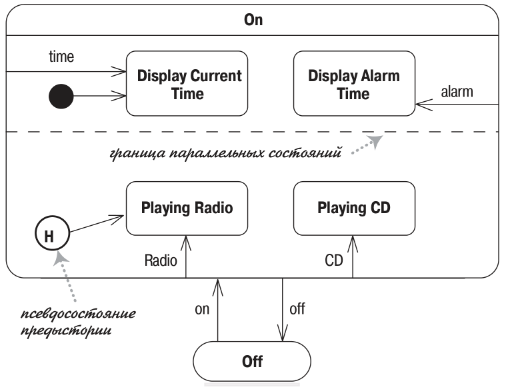
\includegraphics[width=0.7\textwidth]{stateTransitionParallelStates.png}
                \end{center}
            \end{column}
        \end{columns}
    \end{frame}

    \begin{frame}[fragile]
        \frametitle{Генерация кода}
        \begin{columns}
            \begin{column}{0.5\textwidth}
                \begin{tiny}
                    \begin{minted}{java}
public void handleEvent(PanelEvent anEvent) {
    switch (currentState) {
        case PanelState.Open:
            switch (anEvent) {
                case PanelEvent.SafeClosed:
                    currentState = PanelState.Wait;
            }
            break;
        case PanelState.Wait:
            switch (anEvent) {
                case PanelEvent.CandleRemoved:
                    if (isDoorOpen) {
                        revealLock();
                        currentState = PanelState.Lock;
                    }
            }
            break;
        case PanelState.Lock:
            switch (anEvent) {
                case PanelEvent.KeyTurned:
                    if (isCandleIn) {
                        openSafe();
                        currentState = PanelState.Open;
                    } else {
                        releaseKillerRabbit();
                        currentState = PanelState.Final;
                    }
            }
            break;
    }
}
                    \end{minted}
                \end{tiny}
            \end{column}
            \begin{column}{0.5\textwidth}
                \begin{center}
                    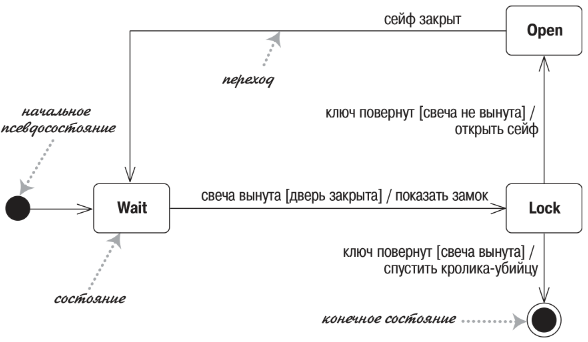
\includegraphics[width=\textwidth]{stateTransitionSyntax.png}
                    \attribution{М. Фаулер, UML. Основы}
                \end{center}
            \end{column}
        \end{columns}
    \end{frame}

    \begin{frame}
        \frametitle{Таблица состояний}
        \begin{center}
            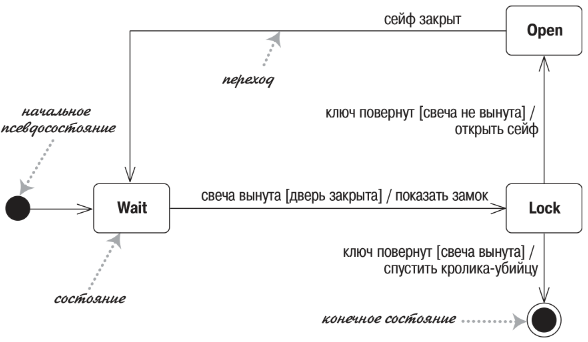
\includegraphics[width=0.4\textwidth]{stateTransitionSyntax.png}
        \end{center}

        \begin{center}
            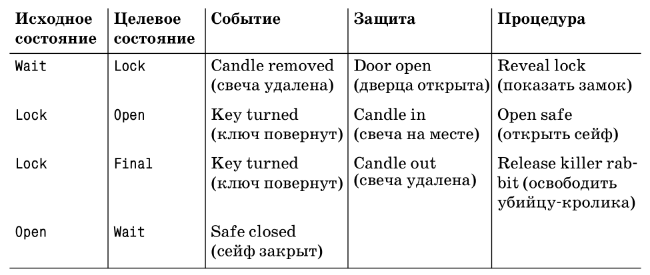
\includegraphics[width=0.5\textwidth]{stateTransitionStateTable.png}
            \attribution{М. Фаулер, UML. Основы}
        \end{center}
    \end{frame}

    \begin{frame}
        \frametitle{Паттерн ``Состояние''}
        \begin{center}
            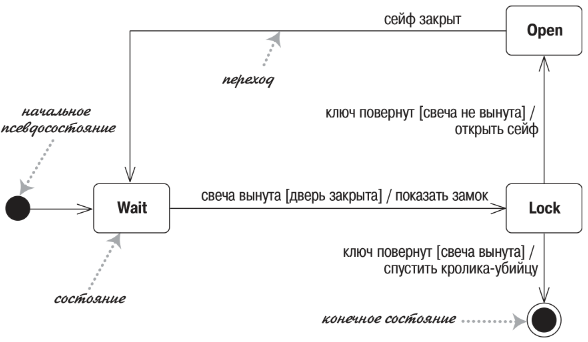
\includegraphics[width=0.4\textwidth]{stateTransitionSyntax.png}
        \end{center}

        \begin{center}
            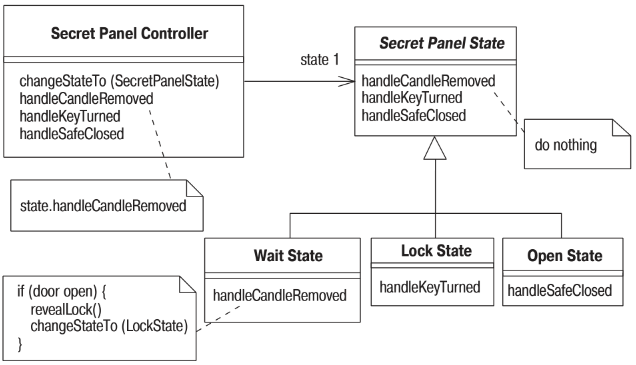
\includegraphics[width=0.5\textwidth]{stateTransitionStatePattern.png}
            \attribution{М. Фаулер, UML. Основы}
        \end{center}
    \end{frame}

    \section{Диаграммы последовательностей}

    \begin{frame}
        \frametitle{Диаграммы последовательностей}
        \begin{columns}
            \begin{column}{0.5\textwidth}
                \begin{itemize}
                    \item Применяются для визуализации взаимодействия между объектами
                    \begin{itemize}
                        \item Особо удобно для асинхронных вызовов
                        \item Телекоммуникационные протоколы
                    \end{itemize}
                    \item Могут применяться на этапе анализа предметной области
                    \item Могут применяться для составления плана тестирования
                    \item И даже для визуализации логов работающей системы
                \end{itemize}
            \end{column}
            \begin{column}{0.5\textwidth}
                \begin{center}
                    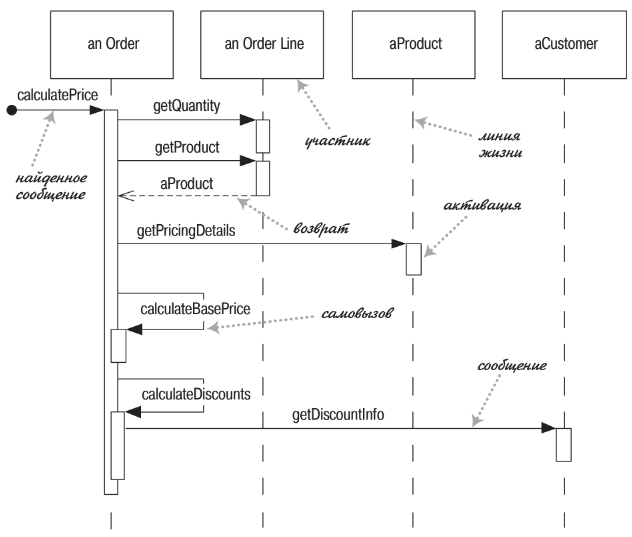
\includegraphics[width=0.9\textwidth]{sequenceDiagramSyntax.png}
                    \attribution{М. Фаулер, UML. Основы}
                \end{center}
            \end{column}
        \end{columns}
    \end{frame}

    \section{Коммуникационные диаграммы}

    \begin{frame}
        \frametitle{Коммуникационные диаграммы}
        \begin{columns}
            \begin{column}{0.5\textwidth}
                \begin{itemize}
                    \item Применяются для визуализации взаимодействия между объектами
                    \begin{itemize}
                        \item Более легковесный аналог диаграмм последовательностей
                        \item Тоже отображают один сценарий взаимодействия
                    \end{itemize}
                \end{itemize}
            \end{column}
            \begin{column}{0.5\textwidth}
                \begin{center}
                    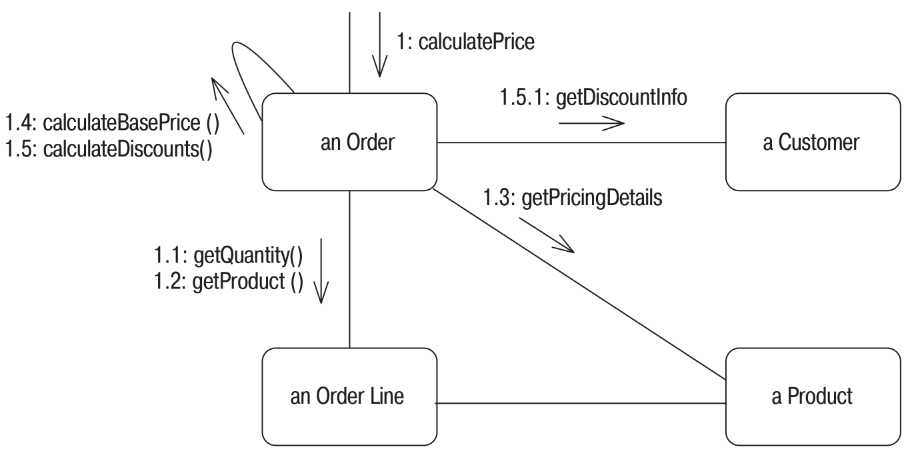
\includegraphics[width=\textwidth]{communicationDiagram.png}
                    \attribution{М. Фаулер, UML. Основы}
                \end{center}
            \end{column}
        \end{columns}
    \end{frame}

    \begin{frame}
        \frametitle{Коммуникационные диаграммы, пример}
        \begin{center}
            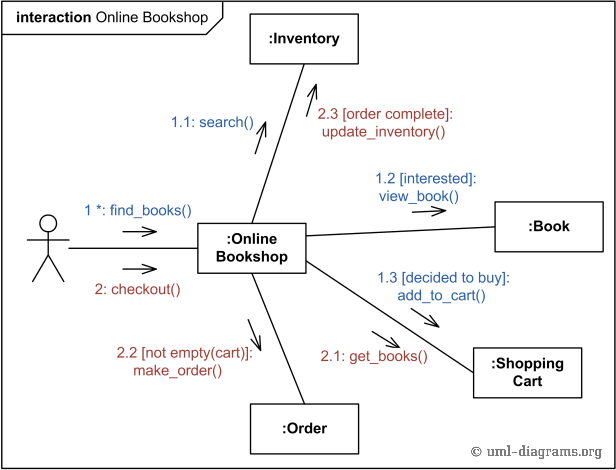
\includegraphics[width=0.6\textwidth]{communicationDiagramExample.png}
            \attribution{http://www.uml-diagrams.org/}
        \end{center}
    \end{frame}

    \section{Диаграммы составных структур}

    \begin{frame}
        \frametitle{Диаграммы составных структур}
        \begin{columns}
            \begin{column}{0.5\textwidth}
                \begin{itemize}
                    \item По сути, продвинутые диаграммы компонентов
                    \item Внутри компоненты не другие компоненты, а части (роли)
                \end{itemize}
                \vspace{3mm}
                \begin{center}
                    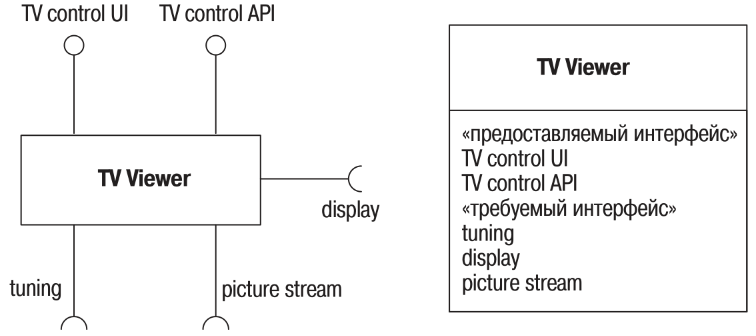
\includegraphics[width=0.9\textwidth]{compositeStructureElement.png}
                \end{center}
            \end{column}
            \begin{column}{0.5\textwidth}
                \begin{center}
                    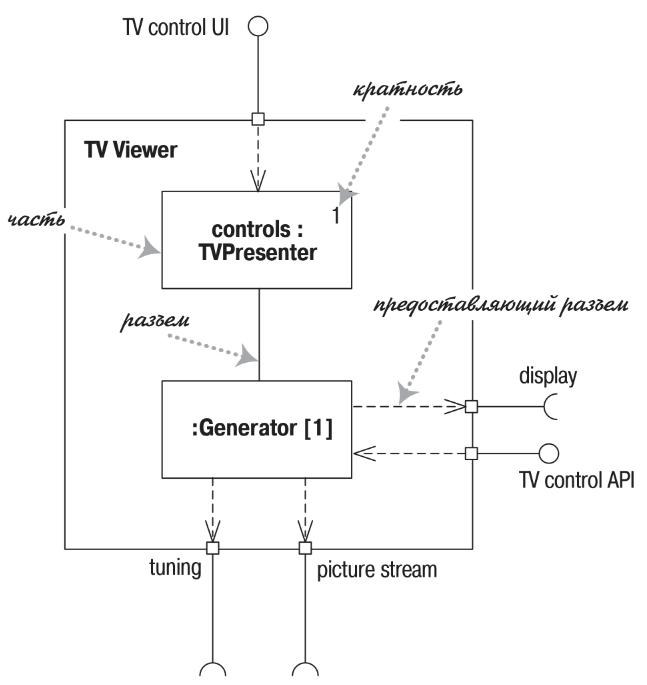
\includegraphics[width=0.8\textwidth]{compositeStructureDiagram.png}
                    \attribution{М. Фаулер, UML. Основы}
                \end{center}
            \end{column}
        \end{columns}
    \end{frame}

    \section{Диаграммы коопераций}

    \begin{frame}
        \frametitle{Диаграммы коопераций}
        \begin{columns}
            \begin{column}{0.5\textwidth}
                \begin{itemize}
                    \item Показывают взаимодействие между объектами (ролями) в рамках одного сценария использования
                \end{itemize}
                \vspace{3mm}
                \begin{center}
                    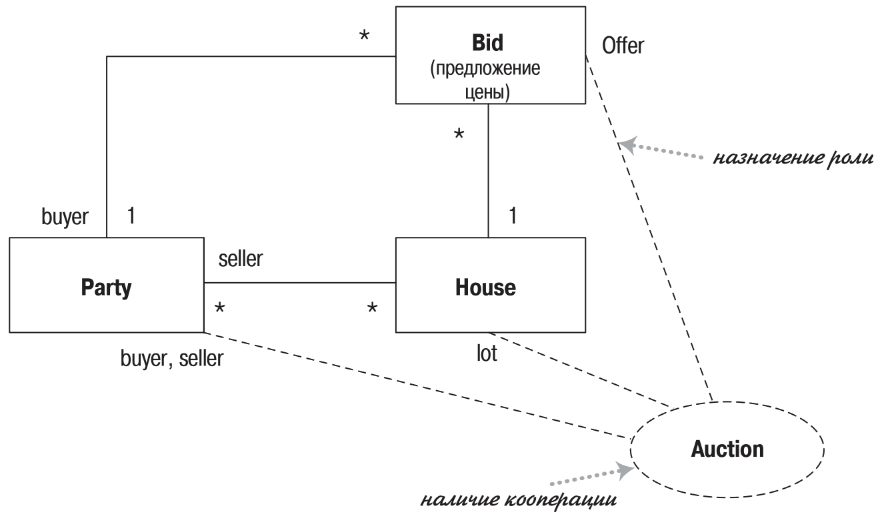
\includegraphics[width=0.9\textwidth]{cooperationAlternateNotation.png}
                \end{center}
            \end{column}
            \begin{column}{0.5\textwidth}
                \begin{center}
                    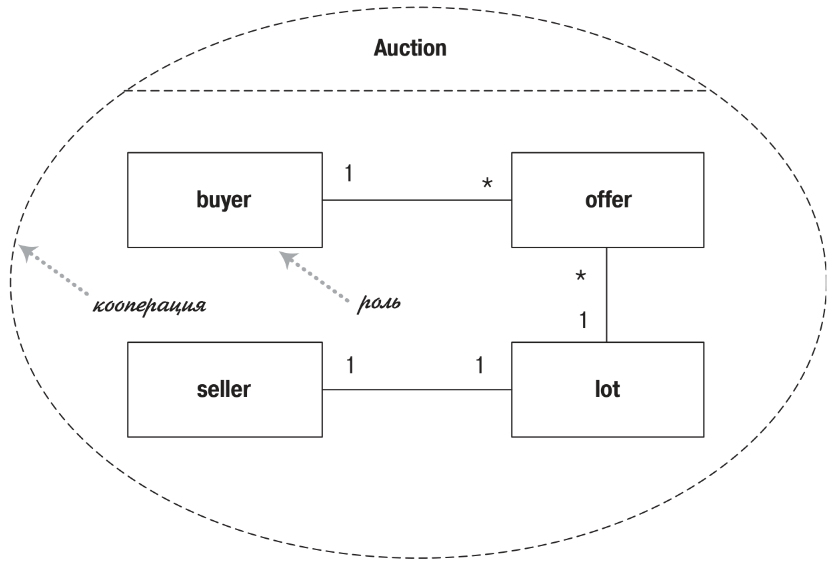
\includegraphics[width=0.9\textwidth]{cooperationDiagram.png}
                    \attribution{М. Фаулер, UML. Основы}
                \end{center}
            \end{column}
        \end{columns}
    \end{frame}

    \section{Временные диаграммы}

    \begin{frame}
        \frametitle{Временные диаграммы}
        \begin{columns}
            \begin{column}{0.5\textwidth}
                \begin{itemize}
                    \item Для моделирования временных ограничений в системах реального времени
                \end{itemize}
                \vspace{3mm}
                \begin{center}
                    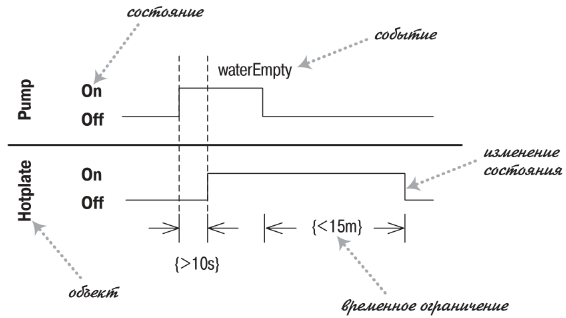
\includegraphics[width=0.9\textwidth]{timingDiagrams.png}
                \end{center}
            \end{column}
            \begin{column}{0.5\textwidth}
                \begin{center}
                    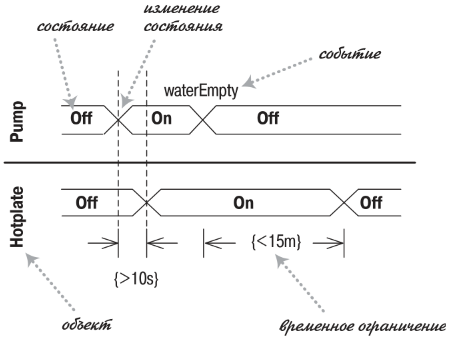
\includegraphics[width=0.8\textwidth]{timingDiagramsAlternate.png}
                    \attribution{М. Фаулер, UML. Основы}
                \end{center}
            \end{column}
        \end{columns}
    \end{frame}

    \begin{frame}
        \frametitle{Временная диаграмма, пример}
        \begin{center}
            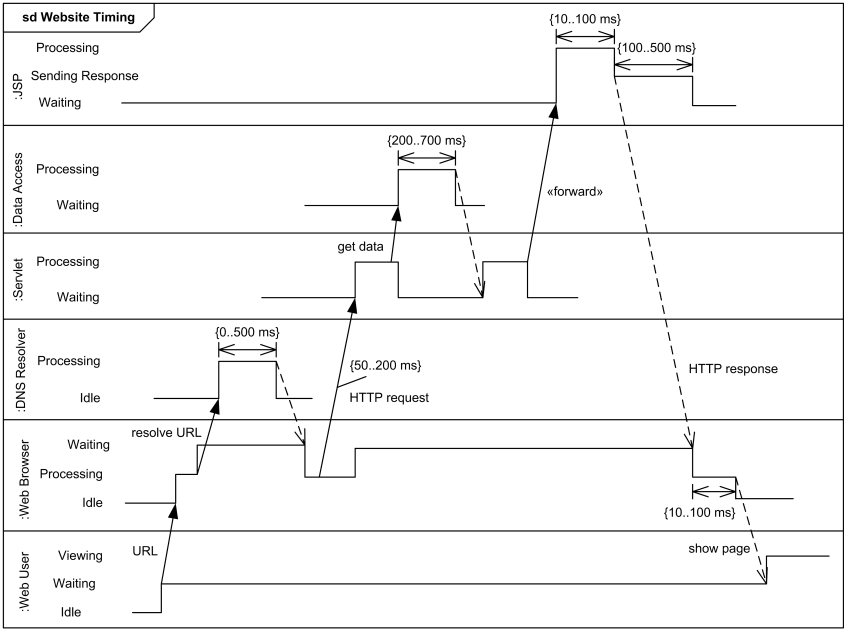
\includegraphics[width=0.7\textwidth]{timingDiagramExample.png}
            \attribution{http://www.uml-diagrams.org/}
        \end{center}
    \end{frame}

    \section{Диаграммы обзора взаимодействия}

    \begin{frame}
        \frametitle{Диаграммы обзора взаимодействия}
        \begin{columns}
            \begin{column}{0.5\textwidth}
                \begin{itemize}
                    \item Диаграммы активностей + диаграммы последовательностей
                    \item Применяются при наличии взаимодействия со сложной логикой, когда фреймы неудобны
                \end{itemize}
            \end{column}
            \begin{column}{0.5\textwidth}
                \begin{center}
                    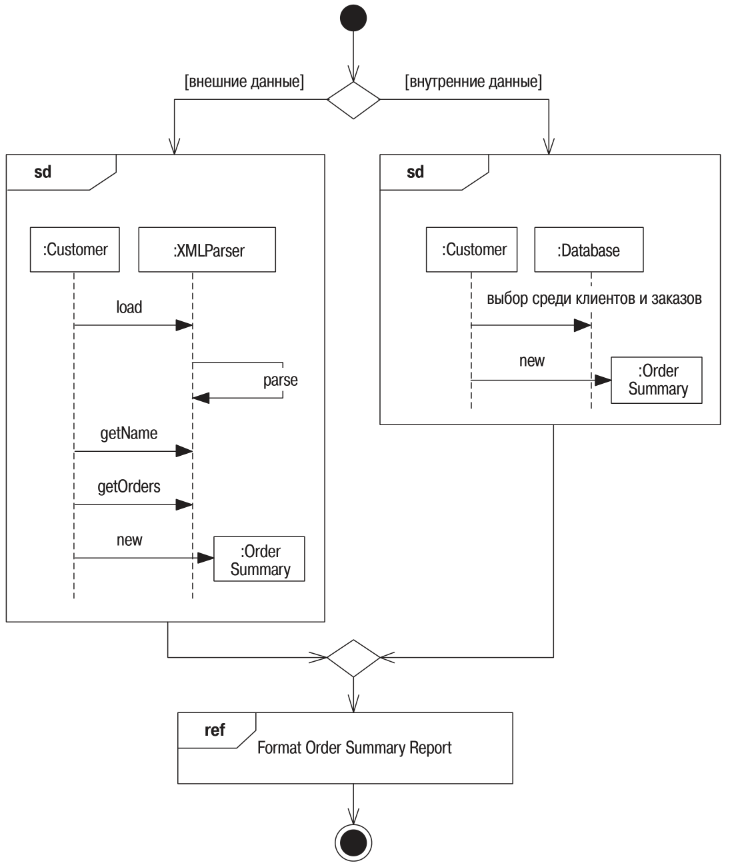
\includegraphics[width=0.9\textwidth]{interactionOverviewDiagrams.png}
                    \attribution{М. Фаулер, UML. Основы}
                \end{center}
            \end{column}
        \end{columns}
    \end{frame}

    \begin{frame}
        \frametitle{Диаграмма обзора взаимодействия, пример}
        \begin{center}
            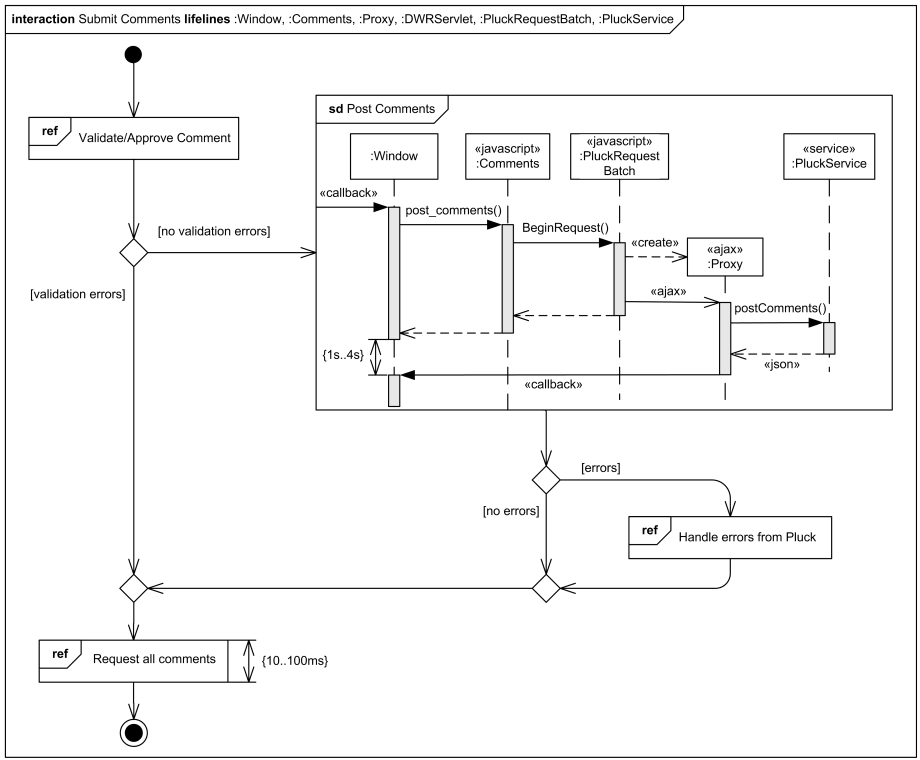
\includegraphics[width=0.7\textwidth]{interactionOverviewExample.png}
            \attribution{http://www.uml-diagrams.org/}
        \end{center}
    \end{frame}

    \section{Диаграммы потоков данных}

    \begin{frame}
        \frametitle{Диаграммы потоков данных}
        \framesubtitle{DFD}
        \begin{columns}
            \begin{column}{0.4\textwidth}
                \begin{itemize}
                    \item Показывают обмен данными в системе
                    \item Внешние сущности, процессы внутри системы, потоки данных
                \end{itemize}
            \end{column}
            \begin{column}{0.6\textwidth}
                \begin{center}
                    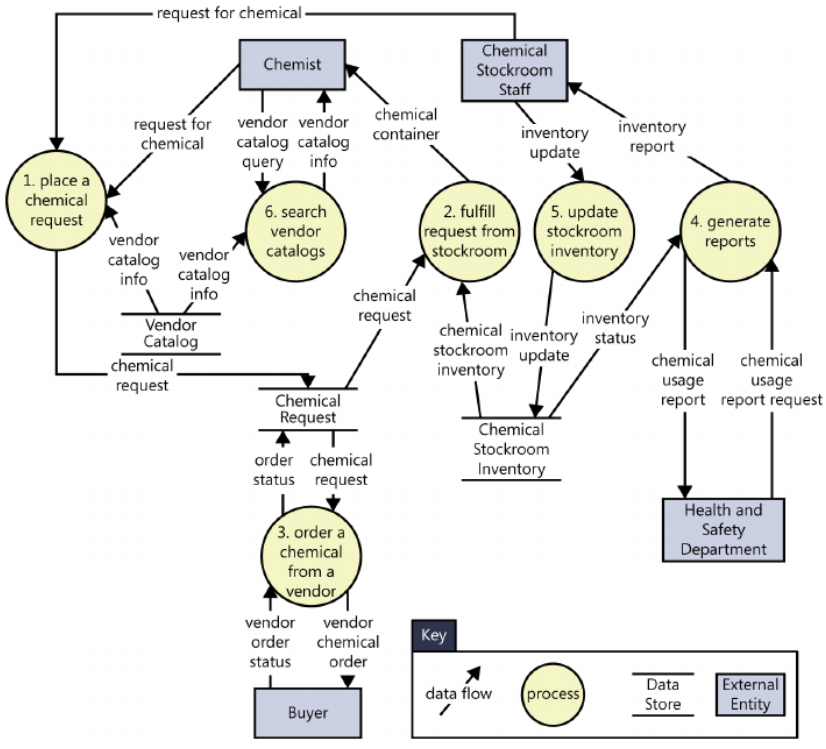
\includegraphics[width=0.9\textwidth]{dfd.png}
                \end{center}
            \end{column}
        \end{columns}
    \end{frame}
    
    \section{Диаграммы IDEF0}
    
    \begin{frame}
        \frametitle{Диаграммы IDEF0}
        \begin{center}
            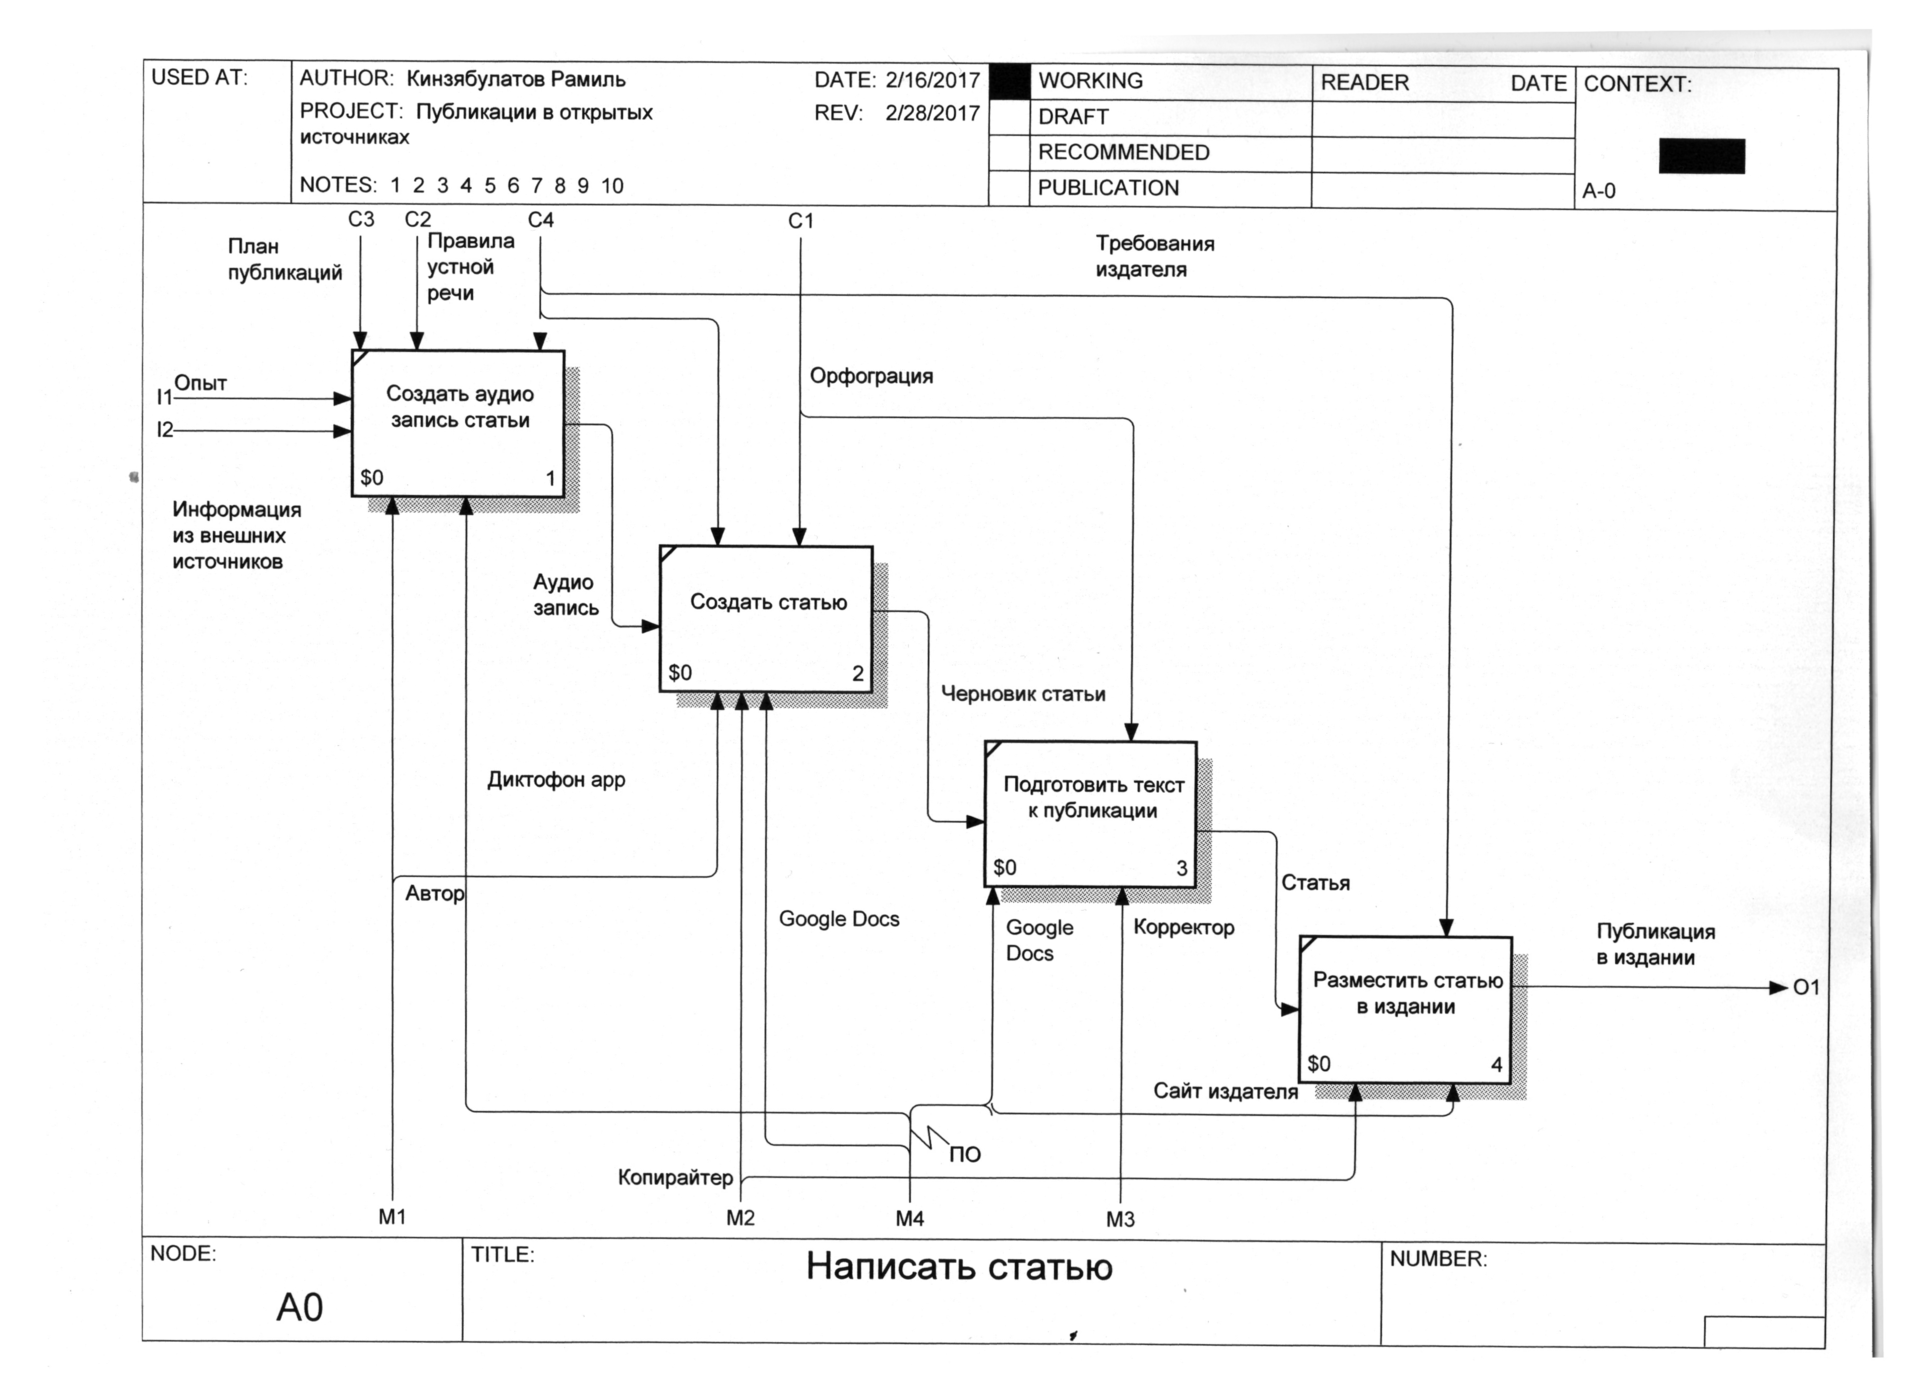
\includegraphics[width=0.80\textwidth]{idef0.png}
            \attribution{https://habrahabr.ru/post/322832/}
        \end{center}
    \end{frame}

    \section{CASE-инструменты}

    \begin{frame}
        \frametitle{Примеры CASE-инструментов}
        \begin{itemize}
            \item ``Рисовалки''
            \begin{itemize}
                \item Visio
                \item Dia
                \item SmartDraw
                \item LucidChart
                \item Creately
                \item Diagrams.Net
            \end{itemize}
            \item Полноценные CASE-системы
            \begin{itemize}
                \item Enterprise Architect
                \item Rational Software Architect
                \item MagicDraw
                \item Visual Paradigm
                \item GenMyModel
            \end{itemize}
            \item Забавные штуки
            \begin{itemize}
                \item \url{https://www.websequencediagrams.com/}
                \item \url{http://yuml.me/}
                \item \url{http://plantuml.com/}
            \end{itemize}
        \end{itemize}
    \end{frame}

    \section{Заключение}

    \begin{frame}
        \frametitle{Книжка}
        \begin{columns}
            \begin{column}{0.5\textwidth}
                \begin{center}
                    
\includegraphics[width=0.4\textwidth]{umlBookCover.png}
                \end{center}
            \end{column}
            \begin{column}{0.5\textwidth}
                М. Фаулер, UML. Основы. Краткое руководство по стандартному языку объектного моделирования. СПб., Символ-Плюс, 2011. 192 С.
            \end{column}
        \end{columns}
    \end{frame}

\end{document}
